% Created by tikzDevice version 0.12 on 2019-03-12 12:51:35
% !TEX encoding = UTF-8 Unicode
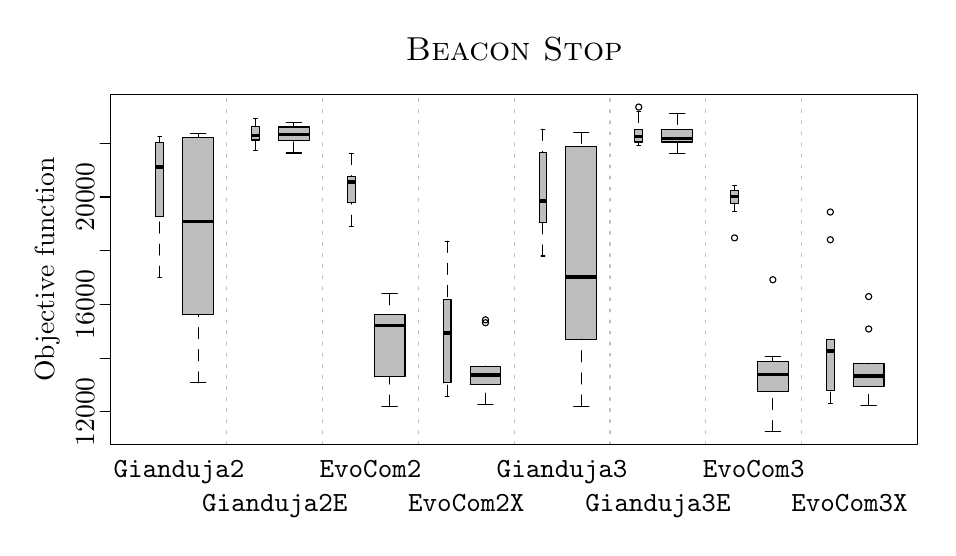
\begin{tikzpicture}[x=1pt,y=1pt]
\definecolor{fillColor}{RGB}{255,255,255}
\path[use as bounding box,fill=fillColor,fill opacity=0.00] (0,0) rectangle (325.21,180.67);
\begin{scope}
\path[clip] ( 30.00, 30.00) rectangle (321.61,156.67);
\definecolor{fillColor}{RGB}{190,190,190}

\path[fill=fillColor] ( 46.34,112.41) --
	( 49.11,112.41) --
	( 49.11,139.15) --
	( 46.34,139.15) --
	cycle;
\definecolor{drawColor}{RGB}{0,0,0}

\path[draw=drawColor,line width= 1.2pt,line join=round] ( 46.34,130.30) -- ( 49.11,130.30);

\path[draw=drawColor,line width= 0.4pt,dash pattern=on 4pt off 4pt ,line join=round,line cap=round] ( 47.72, 90.47) -- ( 47.72,112.41);

\path[draw=drawColor,line width= 0.4pt,dash pattern=on 4pt off 4pt ,line join=round,line cap=round] ( 47.72,141.26) -- ( 47.72,139.15);

\path[draw=drawColor,line width= 0.4pt,line join=round,line cap=round] ( 47.03, 90.47) -- ( 48.42, 90.47);

\path[draw=drawColor,line width= 0.4pt,line join=round,line cap=round] ( 47.03,141.26) -- ( 48.42,141.26);

\path[draw=drawColor,line width= 0.4pt,line join=round,line cap=round] ( 46.34,112.41) --
	( 49.11,112.41) --
	( 49.11,139.15) --
	( 46.34,139.15) --
	( 46.34,112.41);

\path[fill=fillColor] ( 56.03, 76.91) --
	( 67.11, 76.91) --
	( 67.11,140.91) --
	( 56.03,140.91) --
	cycle;

\path[draw=drawColor,line width= 1.2pt,line join=round] ( 56.03,110.58) -- ( 67.11,110.58);

\path[draw=drawColor,line width= 0.4pt,dash pattern=on 4pt off 4pt ,line join=round,line cap=round] ( 61.57, 52.30) -- ( 61.57, 76.91);

\path[draw=drawColor,line width= 0.4pt,dash pattern=on 4pt off 4pt ,line join=round,line cap=round] ( 61.57,142.30) -- ( 61.57,140.91);

\path[draw=drawColor,line width= 0.4pt,line join=round,line cap=round] ( 58.80, 52.30) -- ( 64.34, 52.30);

\path[draw=drawColor,line width= 0.4pt,line join=round,line cap=round] ( 58.80,142.30) -- ( 64.34,142.30);

\path[draw=drawColor,line width= 0.4pt,line join=round,line cap=round] ( 56.03, 76.91) --
	( 67.11, 76.91) --
	( 67.11,140.91) --
	( 56.03,140.91) --
	( 56.03, 76.91);

\path[fill=fillColor] ( 80.96,140.06) --
	( 83.73,140.06) --
	( 83.73,144.90) --
	( 80.96,144.90) --
	cycle;

\path[draw=drawColor,line width= 1.2pt,line join=round] ( 80.96,141.70) -- ( 83.73,141.70);

\path[draw=drawColor,line width= 0.4pt,dash pattern=on 4pt off 4pt ,line join=round,line cap=round] ( 82.34,136.31) -- ( 82.34,140.06);

\path[draw=drawColor,line width= 0.4pt,dash pattern=on 4pt off 4pt ,line join=round,line cap=round] ( 82.34,147.90) -- ( 82.34,144.90);

\path[draw=drawColor,line width= 0.4pt,line join=round,line cap=round] ( 81.65,136.31) -- ( 83.03,136.31);

\path[draw=drawColor,line width= 0.4pt,line join=round,line cap=round] ( 81.65,147.90) -- ( 83.03,147.90);

\path[draw=drawColor,line width= 0.4pt,line join=round,line cap=round] ( 80.96,140.06) --
	( 83.73,140.06) --
	( 83.73,144.90) --
	( 80.96,144.90) --
	( 80.96,140.06);

\path[fill=fillColor] ( 90.65,139.90) --
	(101.73,139.90) --
	(101.73,144.76) --
	( 90.65,144.76) --
	cycle;

\path[draw=drawColor,line width= 1.2pt,line join=round] ( 90.65,141.95) -- (101.73,141.95);

\path[draw=drawColor,line width= 0.4pt,dash pattern=on 4pt off 4pt ,line join=round,line cap=round] ( 96.19,135.38) -- ( 96.19,139.90);

\path[draw=drawColor,line width= 0.4pt,dash pattern=on 4pt off 4pt ,line join=round,line cap=round] ( 96.19,146.43) -- ( 96.19,144.76);

\path[draw=drawColor,line width= 0.4pt,line join=round,line cap=round] ( 93.42,135.38) -- ( 98.96,135.38);

\path[draw=drawColor,line width= 0.4pt,line join=round,line cap=round] ( 93.42,146.43) -- ( 98.96,146.43);

\path[draw=drawColor,line width= 0.4pt,line join=round,line cap=round] ( 90.65,139.90) --
	(101.73,139.90) --
	(101.73,144.76) --
	( 90.65,144.76) --
	( 90.65,139.90);

\path[fill=fillColor] (115.57,117.39) --
	(118.34,117.39) --
	(118.34,127.04) --
	(115.57,127.04) --
	cycle;

\path[draw=drawColor,line width= 1.2pt,line join=round] (115.57,124.85) -- (118.34,124.85);

\path[draw=drawColor,line width= 0.4pt,dash pattern=on 4pt off 4pt ,line join=round,line cap=round] (116.96,108.94) -- (116.96,117.39);

\path[draw=drawColor,line width= 0.4pt,dash pattern=on 4pt off 4pt ,line join=round,line cap=round] (116.96,135.23) -- (116.96,127.04);

\path[draw=drawColor,line width= 0.4pt,line join=round,line cap=round] (116.27,108.94) -- (117.65,108.94);

\path[draw=drawColor,line width= 0.4pt,line join=round,line cap=round] (116.27,135.23) -- (117.65,135.23);

\path[draw=drawColor,line width= 0.4pt,line join=round,line cap=round] (115.57,117.39) --
	(118.34,117.39) --
	(118.34,127.04) --
	(115.57,127.04) --
	(115.57,117.39);

\path[fill=fillColor] (125.27, 54.52) --
	(136.34, 54.52) --
	(136.34, 77.09) --
	(125.27, 77.09) --
	cycle;

\path[draw=drawColor,line width= 1.2pt,line join=round] (125.27, 73.09) -- (136.34, 73.09);

\path[draw=drawColor,line width= 0.4pt,dash pattern=on 4pt off 4pt ,line join=round,line cap=round] (130.81, 43.88) -- (130.81, 54.52);

\path[draw=drawColor,line width= 0.4pt,dash pattern=on 4pt off 4pt ,line join=round,line cap=round] (130.81, 84.49) -- (130.81, 77.09);

\path[draw=drawColor,line width= 0.4pt,line join=round,line cap=round] (128.04, 43.88) -- (133.57, 43.88);

\path[draw=drawColor,line width= 0.4pt,line join=round,line cap=round] (128.04, 84.49) -- (133.57, 84.49);

\path[draw=drawColor,line width= 0.4pt,line join=round,line cap=round] (125.27, 54.52) --
	(136.34, 54.52) --
	(136.34, 77.09) --
	(125.27, 77.09) --
	(125.27, 54.52);

\path[fill=fillColor] (150.19, 52.33) --
	(152.96, 52.33) --
	(152.96, 82.57) --
	(150.19, 82.57) --
	cycle;

\path[draw=drawColor,line width= 1.2pt,line join=round] (150.19, 70.39) -- (152.96, 70.39);

\path[draw=drawColor,line width= 0.4pt,dash pattern=on 4pt off 4pt ,line join=round,line cap=round] (151.58, 47.50) -- (151.58, 52.33);

\path[draw=drawColor,line width= 0.4pt,dash pattern=on 4pt off 4pt ,line join=round,line cap=round] (151.58,103.51) -- (151.58, 82.57);

\path[draw=drawColor,line width= 0.4pt,line join=round,line cap=round] (150.88, 47.50) -- (152.27, 47.50);

\path[draw=drawColor,line width= 0.4pt,line join=round,line cap=round] (150.88,103.51) -- (152.27,103.51);

\path[draw=drawColor,line width= 0.4pt,line join=round,line cap=round] (150.19, 52.33) --
	(152.96, 52.33) --
	(152.96, 82.57) --
	(150.19, 82.57) --
	(150.19, 52.33);

\path[fill=fillColor] (159.88, 51.81) --
	(170.96, 51.81) --
	(170.96, 58.37) --
	(159.88, 58.37) --
	cycle;

\path[draw=drawColor,line width= 1.2pt,line join=round] (159.88, 55.13) -- (170.96, 55.13);

\path[draw=drawColor,line width= 0.4pt,dash pattern=on 4pt off 4pt ,line join=round,line cap=round] (165.42, 44.62) -- (165.42, 51.81);

\path[draw=drawColor,line width= 0.4pt,dash pattern=on 4pt off 4pt ,line join=round,line cap=round] (165.42, 58.37) -- (165.42, 58.37);

\path[draw=drawColor,line width= 0.4pt,line join=round,line cap=round] (162.65, 44.62) -- (168.19, 44.62);

\path[draw=drawColor,line width= 0.4pt,line join=round,line cap=round] (162.65, 58.37) -- (168.19, 58.37);

\path[draw=drawColor,line width= 0.4pt,line join=round,line cap=round] (159.88, 51.81) --
	(170.96, 51.81) --
	(170.96, 58.37) --
	(159.88, 58.37) --
	(159.88, 51.81);

\path[draw=drawColor,line width= 0.4pt,line join=round,line cap=round] (165.42, 75.10) circle (  1.12);

\path[draw=drawColor,line width= 0.4pt,line join=round,line cap=round] (165.42, 74.06) circle (  1.12);

\path[fill=fillColor] (184.81,110.35) --
	(187.58,110.35) --
	(187.58,135.60) --
	(184.81,135.60) --
	cycle;

\path[draw=drawColor,line width= 1.2pt,line join=round] (184.81,118.09) -- (187.58,118.09);

\path[draw=drawColor,line width= 0.4pt,dash pattern=on 4pt off 4pt ,line join=round,line cap=round] (186.19, 98.17) -- (186.19,110.35);

\path[draw=drawColor,line width= 0.4pt,dash pattern=on 4pt off 4pt ,line join=round,line cap=round] (186.19,143.97) -- (186.19,135.60);

\path[draw=drawColor,line width= 0.4pt,line join=round,line cap=round] (185.50, 98.17) -- (186.88, 98.17);

\path[draw=drawColor,line width= 0.4pt,line join=round,line cap=round] (185.50,143.97) -- (186.88,143.97);

\path[draw=drawColor,line width= 0.4pt,line join=round,line cap=round] (184.81,110.35) --
	(187.58,110.35) --
	(187.58,135.60) --
	(184.81,135.60) --
	(184.81,110.35);

\path[fill=fillColor] (194.50, 68.09) --
	(205.58, 68.09) --
	(205.58,137.78) --
	(194.50,137.78) --
	cycle;

\path[draw=drawColor,line width= 1.2pt,line join=round] (194.50, 90.60) -- (205.58, 90.60);

\path[draw=drawColor,line width= 0.4pt,dash pattern=on 4pt off 4pt ,line join=round,line cap=round] (200.04, 43.92) -- (200.04, 68.09);

\path[draw=drawColor,line width= 0.4pt,dash pattern=on 4pt off 4pt ,line join=round,line cap=round] (200.04,142.83) -- (200.04,137.78);

\path[draw=drawColor,line width= 0.4pt,line join=round,line cap=round] (197.27, 43.92) -- (202.81, 43.92);

\path[draw=drawColor,line width= 0.4pt,line join=round,line cap=round] (197.27,142.83) -- (202.81,142.83);

\path[draw=drawColor,line width= 0.4pt,line join=round,line cap=round] (194.50, 68.09) --
	(205.58, 68.09) --
	(205.58,137.78) --
	(194.50,137.78) --
	(194.50, 68.09);

\path[fill=fillColor] (219.43,139.35) --
	(222.19,139.35) --
	(222.19,143.92) --
	(219.43,143.92) --
	cycle;

\path[draw=drawColor,line width= 1.2pt,line join=round] (219.43,141.34) -- (222.19,141.34);

\path[draw=drawColor,line width= 0.4pt,dash pattern=on 4pt off 4pt ,line join=round,line cap=round] (220.81,138.24) -- (220.81,139.35);

\path[draw=drawColor,line width= 0.4pt,dash pattern=on 4pt off 4pt ,line join=round,line cap=round] (220.81,150.36) -- (220.81,143.92);

\path[draw=drawColor,line width= 0.4pt,line join=round,line cap=round] (220.12,138.24) -- (221.50,138.24);

\path[draw=drawColor,line width= 0.4pt,line join=round,line cap=round] (220.12,150.36) -- (221.50,150.36);

\path[draw=drawColor,line width= 0.4pt,line join=round,line cap=round] (219.43,139.35) --
	(222.19,139.35) --
	(222.19,143.92) --
	(219.43,143.92) --
	(219.43,139.35);

\path[draw=drawColor,line width= 0.4pt,line join=round,line cap=round] (220.81,151.98) circle (  1.12);

\path[fill=fillColor] (229.12,139.37) --
	(240.20,139.37) --
	(240.20,143.77) --
	(229.12,143.77) --
	cycle;

\path[draw=drawColor,line width= 1.2pt,line join=round] (229.12,140.70) -- (240.20,140.70);

\path[draw=drawColor,line width= 0.4pt,dash pattern=on 4pt off 4pt ,line join=round,line cap=round] (234.66,135.34) -- (234.66,139.37);

\path[draw=drawColor,line width= 0.4pt,dash pattern=on 4pt off 4pt ,line join=round,line cap=round] (234.66,149.71) -- (234.66,143.77);

\path[draw=drawColor,line width= 0.4pt,line join=round,line cap=round] (231.89,135.34) -- (237.43,135.34);

\path[draw=drawColor,line width= 0.4pt,line join=round,line cap=round] (231.89,149.71) -- (237.43,149.71);

\path[draw=drawColor,line width= 0.4pt,line join=round,line cap=round] (229.12,139.37) --
	(240.20,139.37) --
	(240.20,143.77) --
	(229.12,143.77) --
	(229.12,139.37);

\path[fill=fillColor] (254.04,117.28) --
	(256.81,117.28) --
	(256.81,121.88) --
	(254.04,121.88) --
	cycle;

\path[draw=drawColor,line width= 1.2pt,line join=round] (254.04,119.59) -- (256.81,119.59);

\path[draw=drawColor,line width= 0.4pt,dash pattern=on 4pt off 4pt ,line join=round,line cap=round] (255.43,114.36) -- (255.43,117.28);

\path[draw=drawColor,line width= 0.4pt,dash pattern=on 4pt off 4pt ,line join=round,line cap=round] (255.43,123.70) -- (255.43,121.88);

\path[draw=drawColor,line width= 0.4pt,line join=round,line cap=round] (254.73,114.36) -- (256.12,114.36);

\path[draw=drawColor,line width= 0.4pt,line join=round,line cap=round] (254.73,123.70) -- (256.12,123.70);

\path[draw=drawColor,line width= 0.4pt,line join=round,line cap=round] (254.04,117.28) --
	(256.81,117.28) --
	(256.81,121.88) --
	(254.04,121.88) --
	(254.04,117.28);

\path[draw=drawColor,line width= 0.4pt,line join=round,line cap=round] (255.43,104.71) circle (  1.12);

\path[fill=fillColor] (263.74, 49.26) --
	(274.81, 49.26) --
	(274.81, 59.97) --
	(263.74, 59.97) --
	cycle;

\path[draw=drawColor,line width= 1.2pt,line join=round] (263.74, 55.28) -- (274.81, 55.28);

\path[draw=drawColor,line width= 0.4pt,dash pattern=on 4pt off 4pt ,line join=round,line cap=round] (269.27, 34.69) -- (269.27, 49.26);

\path[draw=drawColor,line width= 0.4pt,dash pattern=on 4pt off 4pt ,line join=round,line cap=round] (269.27, 61.97) -- (269.27, 59.97);

\path[draw=drawColor,line width= 0.4pt,line join=round,line cap=round] (266.50, 34.69) -- (272.04, 34.69);

\path[draw=drawColor,line width= 0.4pt,line join=round,line cap=round] (266.50, 61.97) -- (272.04, 61.97);

\path[draw=drawColor,line width= 0.4pt,line join=round,line cap=round] (263.74, 49.26) --
	(274.81, 49.26) --
	(274.81, 59.97) --
	(263.74, 59.97) --
	(263.74, 49.26);

\path[draw=drawColor,line width= 0.4pt,line join=round,line cap=round] (269.27, 89.59) circle (  1.12);

\path[fill=fillColor] (288.66, 49.69) --
	(291.43, 49.69) --
	(291.43, 68.06) --
	(288.66, 68.06) --
	cycle;

\path[draw=drawColor,line width= 1.2pt,line join=round] (288.66, 63.85) -- (291.43, 63.85);

\path[draw=drawColor,line width= 0.4pt,dash pattern=on 4pt off 4pt ,line join=round,line cap=round] (290.04, 44.93) -- (290.04, 49.69);

\path[draw=drawColor,line width= 0.4pt,dash pattern=on 4pt off 4pt ,line join=round,line cap=round] (290.04, 68.06) -- (290.04, 68.06);

\path[draw=drawColor,line width= 0.4pt,line join=round,line cap=round] (289.35, 44.93) -- (290.74, 44.93);

\path[draw=drawColor,line width= 0.4pt,line join=round,line cap=round] (289.35, 68.06) -- (290.74, 68.06);

\path[draw=drawColor,line width= 0.4pt,line join=round,line cap=round] (288.66, 49.69) --
	(291.43, 49.69) --
	(291.43, 68.06) --
	(288.66, 68.06) --
	(288.66, 49.69);

\path[draw=drawColor,line width= 0.4pt,line join=round,line cap=round] (290.04,104.04) circle (  1.12);

\path[draw=drawColor,line width= 0.4pt,line join=round,line cap=round] (290.04,114.05) circle (  1.12);

\path[fill=fillColor] (298.35, 51.11) --
	(309.43, 51.11) --
	(309.43, 59.18) --
	(298.35, 59.18) --
	cycle;

\path[draw=drawColor,line width= 1.2pt,line join=round] (298.35, 54.83) -- (309.43, 54.83);

\path[draw=drawColor,line width= 0.4pt,dash pattern=on 4pt off 4pt ,line join=round,line cap=round] (303.89, 44.17) -- (303.89, 51.11);

\path[draw=drawColor,line width= 0.4pt,dash pattern=on 4pt off 4pt ,line join=round,line cap=round] (303.89, 59.18) -- (303.89, 59.18);

\path[draw=drawColor,line width= 0.4pt,line join=round,line cap=round] (301.12, 44.17) -- (306.66, 44.17);

\path[draw=drawColor,line width= 0.4pt,line join=round,line cap=round] (301.12, 59.18) -- (306.66, 59.18);

\path[draw=drawColor,line width= 0.4pt,line join=round,line cap=round] (298.35, 51.11) --
	(309.43, 51.11) --
	(309.43, 59.18) --
	(298.35, 59.18) --
	(298.35, 51.11);

\path[draw=drawColor,line width= 0.4pt,line join=round,line cap=round] (303.89, 83.50) circle (  1.12);

\path[draw=drawColor,line width= 0.4pt,line join=round,line cap=round] (303.89, 71.79) circle (  1.12);
\definecolor{drawColor}{RGB}{190,190,190}

\path[draw=drawColor,line width= 0.4pt,dash pattern=on 1pt off 3pt ,line join=round,line cap=round] ( 71.96, 30.00) -- ( 71.96,156.67);

\path[draw=drawColor,line width= 0.4pt,dash pattern=on 1pt off 3pt ,line join=round,line cap=round] (106.57, 30.00) -- (106.57,156.67);

\path[draw=drawColor,line width= 0.4pt,dash pattern=on 1pt off 3pt ,line join=round,line cap=round] (141.19, 30.00) -- (141.19,156.67);

\path[draw=drawColor,line width= 0.4pt,dash pattern=on 1pt off 3pt ,line join=round,line cap=round] (175.81, 30.00) -- (175.81,156.67);

\path[draw=drawColor,line width= 0.4pt,dash pattern=on 1pt off 3pt ,line join=round,line cap=round] (210.42, 30.00) -- (210.42,156.67);

\path[draw=drawColor,line width= 0.4pt,dash pattern=on 1pt off 3pt ,line join=round,line cap=round] (245.04, 30.00) -- (245.04,156.67);

\path[draw=drawColor,line width= 0.4pt,dash pattern=on 1pt off 3pt ,line join=round,line cap=round] (279.66, 30.00) -- (279.66,156.67);
\end{scope}
\begin{scope}
\path[clip] (  0.00,  0.00) rectangle (325.21,180.67);
\definecolor{drawColor}{RGB}{0,0,0}

\node[text=drawColor,anchor=base,inner sep=0pt, outer sep=0pt, scale=  1.00] at ( 54.65, 18.00) {\texttt{Gianduja2}};

\node[text=drawColor,anchor=base,inner sep=0pt, outer sep=0pt, scale=  1.00] at (123.88, 18.00) {\texttt{EvoCom2}};

\node[text=drawColor,anchor=base,inner sep=0pt, outer sep=0pt, scale=  1.00] at (193.12, 18.00) {\texttt{Gianduja3}};

\node[text=drawColor,anchor=base,inner sep=0pt, outer sep=0pt, scale=  1.00] at (262.35, 18.00) {\texttt{EvoCom3}};

\node[text=drawColor,anchor=base,inner sep=0pt, outer sep=0pt, scale=  1.00] at ( 89.26,  6.00) {\texttt{Gianduja2E}};

\node[text=drawColor,anchor=base,inner sep=0pt, outer sep=0pt, scale=  1.00] at (158.50,  6.00) {\texttt{EvoCom2X}};

\node[text=drawColor,anchor=base,inner sep=0pt, outer sep=0pt, scale=  1.00] at (227.73,  6.00) {\texttt{Gianduja3E}};

\node[text=drawColor,anchor=base,inner sep=0pt, outer sep=0pt, scale=  1.00] at (296.97,  6.00) {\texttt{EvoCom3X}};
\end{scope}
\begin{scope}
\path[clip] (  0.00,  0.00) rectangle (325.21,180.67);
\definecolor{drawColor}{RGB}{0,0,0}

\node[text=drawColor,anchor=base,inner sep=0pt, outer sep=0pt, scale=  1.20] at (175.81,168.67) {\textsc{Beacon Stop}};

\node[text=drawColor,rotate= 90.00,anchor=base,inner sep=0pt, outer sep=0pt, scale=  1.00] at (  9.60, 93.34) {Objective function};
\end{scope}
\begin{scope}
\path[clip] (  0.00,  0.00) rectangle (325.21,180.67);
\definecolor{drawColor}{RGB}{0,0,0}

\path[draw=drawColor,line width= 0.4pt,line join=round,line cap=round] ( 30.00, 41.83) -- ( 30.00,138.88);

\path[draw=drawColor,line width= 0.4pt,line join=round,line cap=round] ( 30.00, 41.83) -- ( 26.20, 41.83);

\path[draw=drawColor,line width= 0.4pt,line join=round,line cap=round] ( 30.00, 61.24) -- ( 26.20, 61.24);

\path[draw=drawColor,line width= 0.4pt,line join=round,line cap=round] ( 30.00, 80.65) -- ( 26.20, 80.65);

\path[draw=drawColor,line width= 0.4pt,line join=round,line cap=round] ( 30.00,100.06) -- ( 26.20,100.06);

\path[draw=drawColor,line width= 0.4pt,line join=round,line cap=round] ( 30.00,119.47) -- ( 26.20,119.47);

\path[draw=drawColor,line width= 0.4pt,line join=round,line cap=round] ( 30.00,138.88) -- ( 26.20,138.88);

\node[text=drawColor,rotate= 90.00,anchor=base,inner sep=0pt, outer sep=0pt, scale=  1.00] at ( 24.00, 41.83) {12000};

\node[text=drawColor,rotate= 90.00,anchor=base,inner sep=0pt, outer sep=0pt, scale=  1.00] at ( 24.00, 80.65) {16000};

\node[text=drawColor,rotate= 90.00,anchor=base,inner sep=0pt, outer sep=0pt, scale=  1.00] at ( 24.00,119.47) {20000};

\path[draw=drawColor,line width= 0.4pt,line join=round,line cap=round] ( 30.00, 30.00) --
	(321.61, 30.00) --
	(321.61,156.67) --
	( 30.00,156.67) --
	( 30.00, 30.00);
\end{scope}
\end{tikzpicture}
